\documentclass[10pt,a4paper]{article}
\usepackage[utf8]{inputenc}
\usepackage{amsmath}
\usepackage{amsfonts}
\usepackage{amssymb}
\usepackage{booktabs}
\usepackage{csquotes}
\usepackage{graphicx}
\usepackage{float}
\usepackage{hyperref}
\usepackage{url}

\title{Configurable Radiation Testsuite - Documentation}
\author{Mattis Jaksch}
\date{\today}

\begin{document}
\maketitle

\tableofcontents

\section{Overview}
This testsuite is developed to automate test procedures. It supports different device which can be configured to control the process in a desired way. The interaction between components is realized with the qt-signal-slot mechanism. One may add triggers to a device which are then send out to other devices. For example if the voltage in the Labjack measurement exceeds a certain boundary a signal is send to all the previously selected devices, which could be a power supply switching off to protect the DUT.

	\subsection{Mainwindow}
	
	\begin{figure}[H]
	\centering
	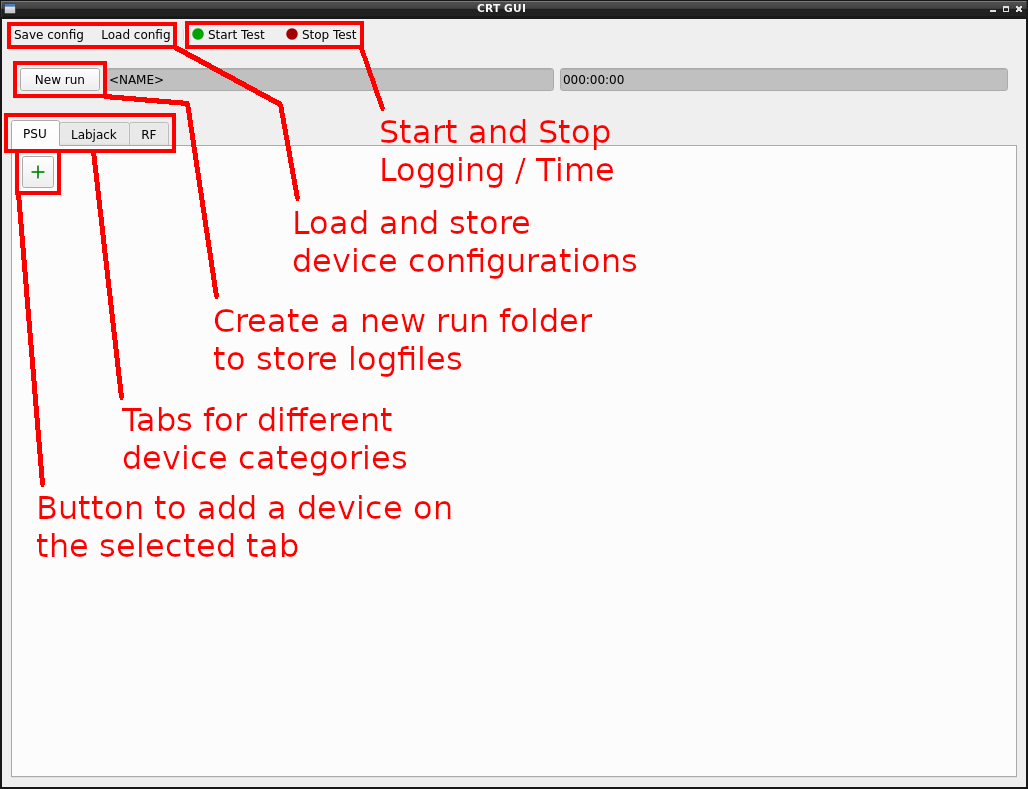
\includegraphics[width=0.9\textwidth]{./1_Plain_Expl.png}
	\caption{Main menu of the suite}
	\end{figure}
	
	On the top row, on the left side, certain configurations for all the components in the various tabs can be either stored or loaded. The stored configuration file is also human readable and editable.
	
	On the right side the test can be started or stopped. Starting and Stopping the test sends a trigger to all components. E.g. the power supply will turn selected channels on/off and start/stop the logging. Therefore one can not click this button twice in a row!
	
	In the row below is the run information. To start a run one should first create a \enquote{New run} by clicking the button and creating a folder to store all the log files. Left of button is the current file location and the time of the run. If one stops the run, the time also halts till the run gets restarted. 
	
	The log files are named after the individual components, so one should make sure to not have any names twice.
	
	\subsection{Testrun}	
	
	\begin{figure}[H]
	\centering
	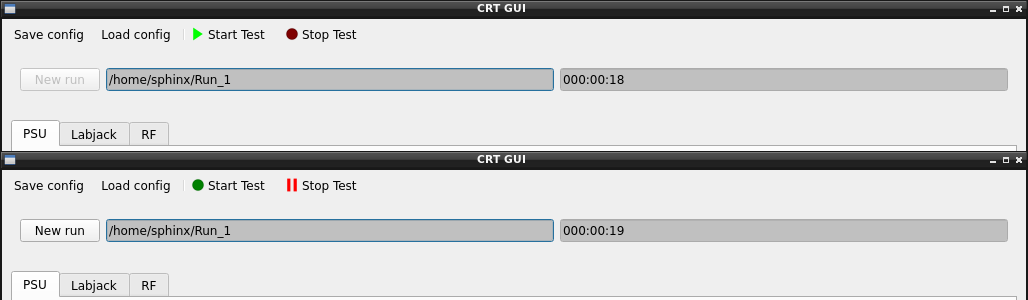
\includegraphics[width=0.9\textwidth]{./4_Testrun.png}
	\caption{An active testrun in the suite}
	\end{figure}
	
	If a test run is started, the \enquote{Start} button and the \enquote{New run} button get deactivated and the time starts to count up. In the background logfiles are generated with a UTC timestamp. The data itself is stored in a \textit{csv} format to be easily readable. To every datapoint or row stored a relative timestamp in milliseconds is added.
	
	To stop the run and therefore the logging and timer the \enquote{Stop} button should be pressed. After that a run can also be continued with by clicking the \enquote{Start} button again.	
	
\section{Components}

	\subsection{Power supply}
	
	\begin{figure}[H]
	\centering
	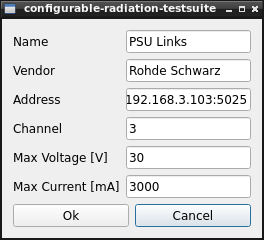
\includegraphics[width=0.5\textwidth]{./2_PSU_menu.png}
	\caption{An active testrun in the suite}
	\end{figure}
	
	The power supply can be either added via configuration file or manually. If it's added manually a small window will pop up. 
	
	In the first row an individual name can be chosen. In the second row the vendor is put in - case insensitive. Then follows the address which has a IP4 part and port after the double dot. In the last three rows a description of the power supply is given with the number of channels and the maximum voltage / current the supply has or someone wants to apply.	
	
		\subsubsection{Supported devices}
		Support for other devices can be easily added. One only needs to edit the \textit{psu.*} files and add a few lines for the correct SCPI\footnote{Standard Commands for Programmable Instruments} Code.
	
		\begin{table}[H]
		\centering
		\begin{tabular}{ll}
		\toprule
		Supplier			& Model \\ \midrule
		Rhode\&Schwarz		& HMC8043 \\
		TTI					& (?) \\
		\bottomrule
		\end{tabular}			
		\end{table}	
	
	\subsection{Labjack}
	
	\begin{figure}[H]
	\centering
	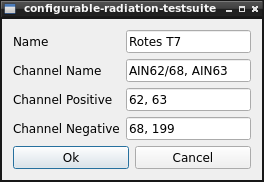
\includegraphics[width=0.5\textwidth]{./3_LBJ_menu.png}
	\caption{An active testrun in the suite}
	\end{figure}
	
	The labjack can be either added via configuration file or manually. If it's added manually a small window will pop up.
	
	In the first row an individual name can be chosen. The channel names in the second row can also be chosen individually. The third and fourth row determines the used channels\footnote{Refer to \url{labjack.com/support/datasheets/t-series/ain}} and if they are differential or not. A differential channel is given by a certain positive and negative address, whereas single ended just use $199$ as negative channel.
	
	
		\subsubsection{Supported devices}
		To support other devices the addresses in the \textit{Labjack.*} files have to be extended.
	
		\begin{table}[H]
		\centering
		\begin{tabular}{ll}
		\toprule
		Supplier			& Model \\ \midrule
		Labjack				& T7 \\
		\bottomrule
		\end{tabular}			
		\end{table}	

	\subsection{RF Signals}
	Not implemented yet
	
		\subsubsection{IIO Daemon}
		
	\subsection{Ethernet}
	Not implemented yet
	

\end{document}